\section{Results}
\label{sec:results}

The tables in this section use FinCall-Surprise, the $\Delta v$ target and the
trading-day definition. MAEC, the level target, MSE, the calendar-day definition
and every other model are in Appendix~\ref{app:complete} and in the supplement,
regenerated from the released CSVs.

% Generated by make_main_tables.py from data/results/result_table_{1,2,4,8}.csv.
\begin{table}[t]
\centering
\footnotesize
\setlength{\tabcolsep}{2.5pt}
\begin{tabular}{lrrrr}
\toprule
Model & $\tau$=3 & $\tau$=7 & $\tau$=15 & $\tau$=30 \\
\midrule
\multicolumn{5}{l}{\textit{Temporal split ($n{=}483$)}}\\
S0 train mean & 0.165 & 0.158 & 0.060 & 0.088 \\
S0 HAR-RV & 0.444 & 0.372 & 0.138 & $-$0.285 \\
S0$'$ past-vol ridge & 0.412 & 0.314 & 0.094 & 0.113 \\
S1 GBDT (ticker FE) & 0.340 & 0.249 & $-$0.126 & $-$0.948 \\
S2 text ridge + vol & 0.333\dag & 0.285 & 0.080 & $-$0.077\dag \\
S3 audio ridge + vol & 0.353\dag & 0.268\dag & 0.033\dag & 0.050\dag \\
S4 stack fusion & 0.406 & 0.347 & 0.066 & 0.100 \\
\midrule
\multicolumn{5}{l}{\textit{Date-ordered disjoint split ($n{=}97$)}}\\
S0 train mean & 0.152 & 0.147 & 0.080 & 0.119 \\
S0 HAR-RV & 0.446 & 0.384 & 0.209 & $-$0.120 \\
S0$'$ past-vol ridge & 0.409 & 0.315 & 0.159 & 0.158 \\
S1 GBDT (ticker FE) & 0.300 & 0.047 & $-$0.324 & $-$1.063 \\
S2 text ridge + vol & 0.160\dag & 0.169\dag & 0.039\dag & $-$0.056\dag \\
S3 audio ridge + vol & 0.312\dag & 0.147\dag & 0.057\dag & 0.098 \\
S4 stack fusion & 0.339\dag & 0.108\dag & $-$0.180\dag & $-$0.028\dag \\
\bottomrule
\end{tabular}
\caption{\textbf{The ladder on FinCall-Surprise.} \Rtwo{} vs.\ persistence on
$\Delta v$ (test). Persistence is 0 by construction. The second block keeps test
companies out of training and the split in date order. One
canonical model per stage (the Stage-3 ridge uses WavLM and eGeMAPS). Each
content cell is tested against the
past-volatility ridge S0$'$ on the same calls. A dagger marks a 95\% interval of
the relative MSE reduction, resampled by company, that lies below the
2\% margin fixed in advance, an asterisk one that lies above it, and an unmarked
cell is inconclusive (Appendix Table~\ref{tab:increment}). The full grid, MAEC,
level-$v$, MSE and the MLP heads are in Appendix~\ref{app:complete}.}
\label{tab:grid}
\end{table}


\paragraph{The baseline to beat.}
HAR-RV is strong everywhere except one cell (Table~\ref{tab:grid}). On the FinCall
temporal split at $\tau{=}30$, the training period includes the COVID spike and
the test year (2021) is calm. There, every long-horizon forecast of the volatility
level does worse than persistence, ours and every content model alike. The same
models do fine on the \tickerdisjoint{} split and on MAEC, so we treat this as a
regime effect and note it. GARCH(1,1) beats HAR-RV at every temporal horizon
(Appendix Table~\ref{tab:baselines}). The reference for every content claim below
is the past-volatility ridge S0$'$, which sees the same price inputs as each
content model and nothing else.

\paragraph{Text models mostly read the company (Table~\ref{tab:controls}, Figure~\ref{fig:swaps}).}
Adding text features to the past-volatility ridge makes it \emph{worse} in all
eight cells of Table~\ref{tab:grid}. The paired test finds no meaningful benefit
in six and no improvement in any. A linear probe recovers the ticker from the
frozen call embedding 89.5\% of the time on FinCall and 53.9\% on MAEC. On the
temporal split, where test companies also appear in training, giving each test
call the transcript of \emph{another call by the same company} changes the score
by less than 0.03, while a random transcript hurts. On the \tickerdisjoint{}
split the same-company swap does hurt at $\tau\ge15$, some call-specific
sensitivity, but that split is not in date order, and on the date-ordered
company-disjoint split the real transcript scores no better than either swap. On MAEC the same-company swap
also moves the score by 0.02 or less, and adding text to the past-volatility
ridge lowers \Rtwo{} in all twelve cells of its three splits.

% Generated by make_main_tables.py from four controls CSVs.
\begin{table}[t]
\centering
\scriptsize
\setlength{\tabcolsep}{3pt}
\begin{tabular}{lrr}
\toprule
Identity probe (linear, frozen call embedding) & accuracy & $\times$chance \\
\midrule
BGE-M3 text, FinCall (357 tickers) & 89.5\% & 319$\times$ \\
BGE-M3 text, MAEC (902 tickers) & 53.9\% & 487$\times$ \\
WavLM audio, FinCall (356 tickers) & 76.3\% & 271$\times$ \\
emotion2vec+ audio, FinCall (356 tickers) & 29.4\% & 105$\times$ \\
\bottomrule
\end{tabular}

\vspace{0.2em}
\begin{tabular}{lrrrr}
\toprule
Content swap (\Rtwo{} on $\Delta v$) & $\tau$=3 & $\tau$=7 & $\tau$=15 & $\tau$=30 \\
\midrule
\multicolumn{5}{l}{\textit{Text ridge, temporal split}}\\
\quad real & 0.182 & 0.202 & 0.044 & $-$0.133 \\
\quad same-company swap & 0.174 & 0.194 & 0.047 & $-$0.110 \\
\quad random swap & 0.145 & 0.110 & 0.008 & $-$0.152 \\
\multicolumn{5}{l}{\textit{Text ridge, date-ordered company-disjoint}}\\
\quad real & 0.122 & 0.133 & 0.009 & $-$0.092 \\
\quad same-company swap & 0.136 & 0.139 & 0.019 & $-$0.057 \\
\quad random swap & 0.173 & 0.166 & 0.084 & 0.099 \\
\bottomrule
\end{tabular}
\caption{\textbf{Identity checks.} Frozen embeddings identify the company far
above chance. Where companies recur (temporal), giving a test call another call
by the \emph{same} company barely changes the text model, while a random call
hurts. On the date-ordered company-disjoint split the real transcript scores no
better than either swap. The audio swaps are in Appendix Table~\ref{tab:audio}.}
\label{tab:controls}
\end{table}


\begin{figure*}[t]
\centering
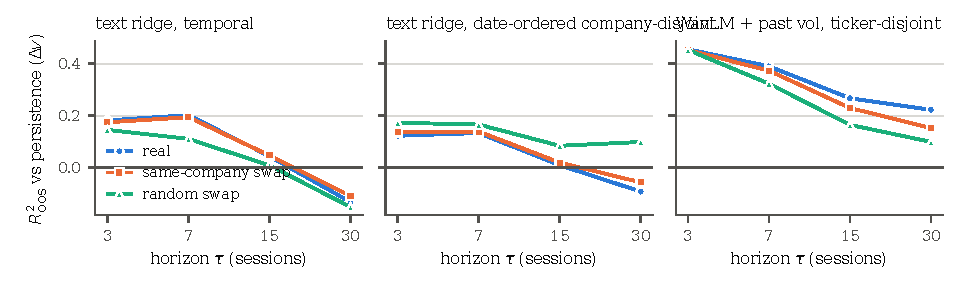
\includegraphics[width=\textwidth]{figures/fig_swaps.pdf}
\caption{\textbf{Content swaps.} \Rtwo{} vs.\ persistence on $\Delta v$ (test) when
each test call keeps its own transcript or audio (real), receives another call by
the same company, or receives a random call. Where companies recur in training
(left), the same-company swap leaves the text model unchanged. On the date-ordered
company-disjoint split (middle) the real transcript does no better than either
swap. The audio model with past volatility (right, \tickerdisjoint{} split) keeps
its score under a random swap at $\tau{=}3$.
Data from Table~\ref{tab:controls}.}
\label{fig:swaps}
\end{figure*}

\paragraph{Audio adds nothing to past volatility.}
Audio-only ridges on eGeMAPS, WavLM-Large and emotion2vec+ stay within 0.10 of the
constant at every horizon (Appendix Table~\ref{tab:audio}) and never beat it by
more than 0.02. Adding WavLM and eGeMAPS to the past-volatility ridge makes it
worse in all eight cells, with no meaningful benefit in seven. In the
audio-swap check (Appendix Table~\ref{tab:audio}), the model with past volatility
keeps its score at $\tau{=}3$ when every test call is given a \emph{random other
company's} audio (0.456 to 0.453). At longer horizons the swap costs more, but
the model with real audio stays below the ridge with past volatility alone. A
probe still recovers the ticker from pooled WavLM embeddings 76.3\% of the time. A pitch-proxy
gender check finds a small gap (test MSE 0.243 against 0.239), a limited
diagnostic rather than a measured demographic. Rerun on Earnings25 by bitrate, the gain from real over randomly swapped
audio never exceeds 0.03, is negative in 7 of 12 cells, and is no larger at
64\,kbps than at lower bitrates (Appendix Table~\ref{tab:earnings25-audio}), a
consistency across observed groups rather than a controlled codec test.

\paragraph{Combining modalities.}
Gated fusion is below the ridge heads with past volatility in 15 of 16 temporal
and \tickerdisjoint{} cells. The
stacking model is the best content model. Against the past-volatility ridge it
shows no meaningful benefit in all four date-ordered company-disjoint cells and is
inconclusive in the four temporal ones. Its one apparent gain is on the
\tickerdisjoint{} split at $\tau{=}30$, which is not in date order. There it
reduces MSE by 11\% against the past-volatility ridge, with an interval from 1\%
to 20\% that is inconclusive under the margin, and by 8\% against HAR-RV, with an
interval that includes zero (Appendix Table~\ref{tab:increment}). The forward-looking
target lifts that cell above the margin, while on the date-ordered split the same
model is 25\% worse. The condition we set in advance for a positive paper, gains
surviving the checks on at least two of four horizons, was not met.

\paragraph{Published models under the checks (Table~\ref{tab:repro-main}, Figure~\ref{fig:repro}).}
Among the five papers we could run, the results that reproduce belong to
price-only or same-company models (Appendix~\ref{app:repro} separates direct
reproductions, repaired runs and ports). Same-Company-Same-Signal reproduces from
its shipped data, and KeFVP, a price-series model conditioned on text,
reproduces seven of eight MAEC cells. HTML's released code does not reproduce its published table,
and the published ensemble of \citet{sawhney2020mm} is matched only through its
finance branch, with mixing weights chosen on the test set. DialogueGAT's corpus
was never released, so it is ported to FinCall. Holding companies out raises the
MSE of the three text models by 12--82\%, while TSMixer and KeFVP move by
$-$10\% to $+$7\% with no consistent sign. The SCSS and KeFVP comparisons use the
same test calls. The HTML and ensemble ones do not, so they also reflect a change
of test set. Training-set size is an unlikely explanation, since the held-out
training sets are as large (EC) or cut by the same third (DEC, MAEC) for both
groups, though only a matched removal of unrelated companies would settle it. The
training-test gap moves models by at most 13\%. HTML's own
trained model changes by at most 4\% when a test transcript is swapped for
another call by the same company, against 9--23\% for a different company's call.

% Generated by make_main_tables.py from the values in tables/repro_controls.tex.
\begin{table}[t]
\centering
\scriptsize
\setlength{\tabcolsep}{3pt}
\begin{tabular}{lrrrr}
\toprule
Model (data), change in test MSE & $\tau$=3 & $\tau$=7 & $\tau$=15 & $\tau$=30 \\
\midrule
\multicolumn{5}{l}{\textit{Companies held out (\tickerdisjoint{} vs.\ the model's own split)}}\\
HTML text (EC) & +18\% & +55\% & +55\% & +82\% \\
HTML text$+$audio (EC) & +20\% & +44\% & +61\% & +70\% \\
Sawhney ensemble (EC) & +13\% & +28\% & +41\% & +38\% \\
SCSS TMLP, text (DEC) & +12\% & +23\% & +25\% & +27\% \\
SCSS TSMixer, price (DEC) & +7\% & +5\% & $-$6\% & $-$8\% \\
KeFVP, text$+$price (MAEC-15) & $-$3\% & +4\% & +3\% & $-$1\% \\
KeFVP, text$+$price (MAEC-16) & $-$9\% & $-$3\% & $-$10\% & $-$4\% \\
\midrule
\multicolumn{5}{l}{\textit{30-session embargo vs.\ the model's own split}}\\
HTML text (EC) & +10\% & +3\% & $-$3\% & +11\% \\
Sawhney ensemble (EC) & +5\% & $-$6\% & $-$2\% & $-$9\% \\
SCSS TMLP (DEC) & $-$4\% & +1\% & 0\% & +3\% \\
\midrule
\multicolumn{5}{l}{\textit{HTML text, transcript replaced by (own split, 97 calls)}}\\
another call, \emph{same} company & +1\% & +4\% & +3\% & +2\% \\
a call of a \emph{different} company & +9\% & +11\% & +21\% & +23\% \\
\bottomrule
\end{tabular}
\caption{\textbf{The field's runnable models under our controls} (Result
Table~6R-C). Each row keeps the configuration of Appendix Table~\ref{tab:faithful}
and changes only the split. Holding companies out costs every text model 12--82\%
and leaves the price-dominated models unchanged, with held-out training sets as
large (EC) or cut by the same third (DEC, MAEC). Absolute values are in Appendix
Table~\ref{tab:repro-controls}.}
\label{tab:repro-main}
\end{table}


\begin{figure}[t]
\centering
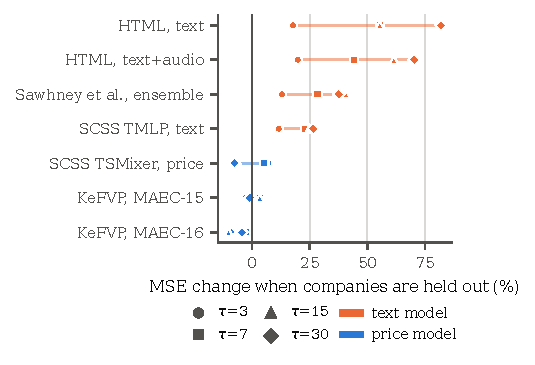
\includegraphics[width=\linewidth]{figures/fig_repro.pdf}
\caption{\textbf{Published models with companies held out.} Change in test MSE
when the same model is scored on a \tickerdisjoint{} split of its own data, one
marker per horizon (data from Table~\ref{tab:repro-main}). The MSE of the three
text models rises by 12--82\%, and the two price-based models show no consistent
change.}
\label{fig:repro}
\end{figure}

\paragraph{After the cutoff (Table~\ref{tab:lookahead}).}
We scored the FinCall-trained models, unchanged, on 475 Earnings25 calls from late
2025, after every model's training cutoff. 280 of those companies (59\%) appear
in FinCall's training split four years earlier, so this is a later cohort, not
an unseen one. On the
level target, no model that was competitive before the cutoff got worse. HAR-RV
rose from 0.44, 0.37, 0.14 and $-$0.29 to 0.60, 0.54, 0.35 and 0.08, and the
content ridges rose with it (only the fusion ridge is unstable, at $\tau{=}30$).
Levels are not comparable across the cutoff, but the ordering is, and it holds.
HAR-RV beats every content model at every horizon. Refit under the call-date anchor of the published label sets,
the same models collapse before the cutoff. Text plus past volatility on
$\Delta v$ falls to between $-1.7$ and $-3.6$ at 3 to 15 days (Appendix
Table~\ref{tab:lookahead-assumed}), because the reaction session then sits inside
the past-volatility features.

% Generated by make_main_tables.py from data/results/result_table_7.csv.
% Level-v target, R^2_OOS vs persistence; in = FinCall temporal test (2021, in-cutoff),
% post = 475 Earnings25 calls (Jul-Dec 2025), same frozen heads, no retraining.
\begin{table}[t]
\centering
\scriptsize
\setlength{\tabcolsep}{2.5pt}
\begin{tabular}{lrrrr}
\toprule
Head (in-cutoff $\to$ post-cutoff) & $\tau$=3 & $\tau$=7 & $\tau$=15 & $\tau$=30 \\
\midrule
S0 train mean & 0.36$\to$0.58 & 0.14$\to$0.47 & $-$0.37$\to$0.15 & $-$1.05$\to$$-$0.29 \\
S0 HAR-RV & 0.44$\to$0.60 & 0.37$\to$0.54 & 0.14$\to$0.35 & $-$0.29$\to$0.08 \\
S2 text ridge + vol & 0.43$\to$0.57 & 0.34$\to$0.50 & 0.03$\to$0.25 & $-$0.45$\to$$-$0.20 \\
S3 WavLM ridge + vol & 0.38$\to$0.57 & 0.24$\to$0.43 & $-$0.09$\to$0.15 & $-$0.66$\to$$-$0.32 \\
S4 fusion ridge + vol & 0.41$\to$0.50 & 0.32$\to$0.46 & $-$0.02$\to$0.20 & $-$0.63$\to$$-$1.93 \\
\bottomrule
\end{tabular}
\caption{\textbf{Frozen-pipeline post-cutoff evaluation} (Result Table~7).
Heads fit once on FinCall's training split, scored unchanged in-cutoff (the 2021
FinCall test year) and post-cutoff (475 Earnings25 calls, late 2025); level-$v$,
\Rtwo{} vs.\ persistence. No head competitive in-cutoff degrades; the ordering survives, with
HAR-RV above every content head at every horizon. Month-cluster bootstrap CIs and
$\Delta v$ rows are in the released CSV.}
\label{tab:lookahead}
\end{table}

